Der Abzug soll das Material aus dem Rohrofen abführen und die Faser in geeigneter Art und Weise für die Weiterverarbeitung auswerfen.
 \vspace{2mm}
\begin{enumerate}
    \item[]Die folgenden Bedingungen aus der Anforderungsliste sind zu erfüllen: \vspace{2mm}
    \item Die Dicke der abzuziehenden Faser soll je nach Material zwischen $200\mu m$ und  $ 2mm$ einstellbar sein (Tabelle \ref{tab:anforderungsliste} Punkt 5.1). Dabei ist zu beachten das aufgrund verschiedener Fließeigenschaften der Kunststoffe nicht alle Dicken des Bereichs erreichbar sind.
    \item Zur einfachen Weiterverarbeitung soll die Faser auf eine wechselbare Standardisierte Spule aufgewickelt werden (Tabelle \ref{tab:anforderungsliste} Punkt 5.2), welche sich einfach austauschen lässt (Tabelle \ref{tab:anforderungsliste} Punkt 5.3).
\end{enumerate}



\subsection{Varianten}
\begin{enumerate}[label=(\alph*)]

   \item \textbf{Aufrollen auf eine Spule} \label{Aufrollen_auf_eine Spule}\\
    Die abtropfende Faser wird unterhalb des Rohrs aufgefangen und direkt auf eine Spule aufgewickelt (Abbildung: \ref{fig:aufrollen}). Zur Einhaltung der angeforderten Standartspule wird für diese ein Außendurchmesser von $100mm$ angenommen. Die benötigte Motordrehzahl ist direkt vom Spulendurchmesser (Gl. (\ref{eq:drehzahlband_1})) abhängig.
    \begin{equation}\label{eq:drehzahlband_1}
        n = \frac{v}{ \pi * d} \hspace{3mm}\hspace{3mm} 
    \end{equation}
    Somit ergibt sich mittels Gleichung \ref{eq:drehzahlband_1}  das  benötigte Drehzahlband.
    \begin{equation*}
        n = [0,191;95,453]\frac{1}{min} 
    \end{equation*}
  
    Da die Drehzahlen sehr gering sind und davon ausgehen ist das es die benötigte Abzugskraft ebenfalls ist,ist ein Direktantrieb der Spule denkbar. In diesem Fall ist das aus der Beschleunigung der Spule hervorgehende Drehmoment das welches überwiegt. Diese Variante bringt aber auch einige Probleme mit sich. Zunächst ist die Steuerung der Abzugsgeschwindigkeit nicht ganz trivial. Die Antriebsgeschwindigkeit muss aufgrund des steigendes Spulendurchmessers während des Wickelns im laufe des Prozesses reduziert werden. Problematisch dabei ist den Aktuellen Spulendurchmesser zu bestimmen da dieser sowohl von dem Durchmesser der Faser als auch von  seiner Verteilung auf der Spule abhängt. Eine Weitere Herrausforderung ist der Start des Prozesses. So muss zu beginn die Faser auf die Spule aufgebracht werden um überhaupt einen Zug auf die Faser ausüben zu können. Alles in allem bedeutet die das Voraussetzung für für eine gute Regelbarkeit dieser Variante ist, das es eine Möglichkeit gibt die Faser initial in die Spule einzuhängen und das diese dann gleichmäßig über die Länge  verteilt wird.  
   
 
    \item \textbf{Abtriebsrollen} \label{abtriebsrollen_c}\\
    Die Faser wird unterhalb des Heizrohrs zwischen zwei relativ kleine Rollen geklemmt, welche sie vom Halbzeug abziehen (Abbildung: \ref{fig:abtreiben}). Die Berechnung erfolgt anlago zu \ref{Aufrollen_auf_eine Spule}. Nur der Spulendurchmesser ist nun der Rollendurchmesser, welcher auf $10mm$ festgelegt wird. Das Drehzahlaband für den Motor, in diesem Fall, ergibt sich somit wie folgt.
    \begin{equation*}
        n = [1,910;954,9230]\frac{1}{min}
    \end{equation*}
    Zu erkennen ist direkt das die Benötigten Drehzahlen um den Faktor 10 größer sind, da die Werte jedoch nicht zu groß sind ist dies zunächst kein Punkt, der der Variante negativ ausgelegt werden kann. Anzumerken ist aber das die Rollen die Faser mit geeigneter Kraft klemmen müssen damit gezogen werden kann. Dabei darf die Anpresskraft jedoch nicht so groß sein das es zu einer Beschädigung der Faser kommt. Da Verschiedenen Materialeien mit diversen Festigkeiten verwedet werden könnten ist die Kraft dem aktuellen Bedingungen immer anzupassen. Die Ermittlung der jeweils benötigten kraft ist Vermutlich nur durch Versuche möglich, da die Faser aus mehreren Materialien besteht und sich ja nach Rotation um ihre Längsachse  unterschiedlich verhalten kann. Zudem sollten beide Räder Angetrieben sein um die Reibung auf der Faser zu minimieren. 
    

     \begin{figure}[!h]
     \centering
     \begin{subfigure}[]{5cm}
         \centering
         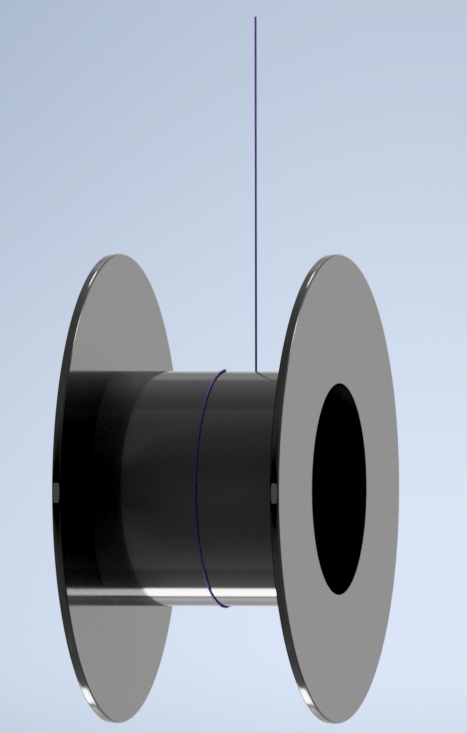
\includegraphics[width=\textwidth]{Abbildungen/aufrollen.png}
         \caption{}
         \label{fig:aufrollen}
     \end{subfigure}
     \hspace{10mm}
     \begin{subfigure}[]{5.4cm}
         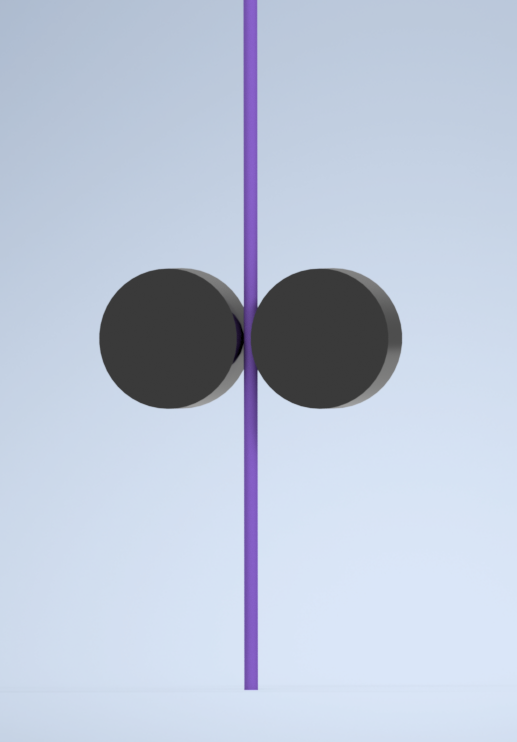
\includegraphics[width=\textwidth]{Abbildungen/abtriebsrollen.png}
         \caption{}
         \label{fig:abtreiben}
     \end{subfigure}
     \caption{Abzugsvarianten}
      \label{fig:abzugsvarianten}
        \end{figure}
        
   

    \item \textbf{Auswahl}\\
    Beide Varianten haben in gewissen Bereichen Vorteile und in anderen Nachteile. Jedoch gibt es bei Variante \ref{abtriebsrollen_c} den entscheidenden Nachteil das nach dem Abtreiben die Faser nirgends aufgenommen wird. Das führt dazu, das mit einer zusätzlichen Baugruppe, eine Lösung geschaffen werden muss. Da die naheliegende Möglichkeit der Aufnahme, der Faser, das Aufrollen ist, wären bei diesem Ansatz die Komponenten von Variante \ref{Aufrollen_auf_eine Spule} zusätzlich vonnöten. Aus diesem Grund werden die Nachteile von Variante \ref{Aufrollen_auf_eine Spule} in kauf genommen. Da diese Art der Konstruktion ebenfalls simpler und mit einem niedrigeren Drehzahlband einhergeht ist sie für einen Prototypen am geeignetsten. Sollte sich während der Konstruktion und Erprobung herausstellen das die Geschwindigkeitssteurung in diesem Fall zu instabil ist, können die Abtriebsrollen nachgerüstet werden.
    
\end{enumerate}
\newpage

\subsection{Dimensionierung und Komponentenauswahl}

%\begin{enumerate}[label=(\alph*)]

\subsubsection{Antriebsmoment an der Spule}
Die zum abziehen der Faser benötigten Kräfte sind sehr klein und werden deshalb im nachfolgenden vernachlässigt. Somit ist das aufzubringende Antriebsmoment ausschließlich von der Massenträgheit und der Beschleunigung abhängig. Um die Berechnung zu vereinfachen wird eine konstante Beschleunigung angenommen. \\
\textit{Weiterhin werden folgende Annahmen getroffen:}
\begin{center}
    \begin{table}[!h]
        \begin{tabular}{ll|ll}
             Maximaldrehzahl & $n_{max}=95,453min^{-1}$ &
             Spulenhöhe & $h=0,07m$ \\
             Spuleninnendurchmesser & $d_i = 0,1m$ &
             Spulenaußendurchmesser & $d_a = 0,2m$\\
             maximale Materialdichte & $\rho = 3000 \frac{kg}{m^3}$ &
             Beschleunigungszeit & $t_0 = 4s$   
        \end{tabular}
    \caption{Kennwerte zur Berechnung des Antriebsmomentes}
    \label{tab:geg_antriebsmoment}
    \end{table}
\end{center}
Die Gleichung \ref{eq:antriebsmoment_aus_trägheit} kann nun zur berechnung verwendet werden. 
\begin{equation}\label{eq:antriebsmoment_aus_trägheit}
     M =  J_P \cdot \Ddot{\varphi}
\end{equation}

Um die Massenträgehit $J_P$ zu berechnen wird in erster Linie nicht die Masse der Spule benötigt. Es ist zwar in der Regel davon auszugehen das die Spule nur leer, zu beginn des Prozesses, beschleunigt werden muss jedoch wird aus Gründen der Flexibilität die Anlage so ausgelegt das die Beschleunigung auch mit voller Spule möglich ist. 
\begin{equation}\label{eq:masse_von_d}
    m = (d_a^2-d_i^2) \cdot \frac{\pi \cdot h \cdot \rho}{4}
\end{equation}
Vereinfacht betrachtet ist die Spule ein Hohlzylinder weshalb die Masse mit Gleichung \ref{eq:masse_von_d} berechnet werden kann. Der äußere Durchmesseer $d_a$ steigt dabei je mehr Faser aufgewickelt wurde. Um auch hier einfach zu bleiben werden die beim aufwickeln entstehenden Freiräume nicht berücksichtigt. 
\begin{equation}\label{eq:polare_Jp}
    J_P = m \cdot \frac{d_a^2+d_i^2}{8}
\end{equation}
So kann mit  Gleichung \ref{eq:polare_Jp} und \ref{eq:masse_von_d} das Polare Massenträgheitsmoment der Spule vollständig beschrieben werden.
\begin{equation}
    J_P = \frac{\pi \cdot h \cdot \rho}{32} \cdot (d_a^4-d_i^4)
\end{equation}

Nun wird noch die Winkelbeschleunigung benötigt, welche sich aus der ersten Ableitung der Winkelgeschwindigkeit ergibt.
\begin{equation}\label{eq:winkelgeschwinigkeit}
    \dot{\varphi} = 2\pi n
\end{equation}
Da die Drehzahl Zeitveränderlich ist kann sie mit den angaben aus Tabelle \ref{tab:geg_antriebsmoment} wie folgt beschrieben werden.
\begin{equation}
    n= \frac{n_{max}}{t_0} \cdot t
\end{equation}
Somit folgt die Winkelbeschleunigung.
\begin{equation}\label{eq:winkelbneschleunigung}
    \Ddot{\varphi} = 2\pi \frac{n_{max}}{t_0}
\end{equation}
Werden jetzt alles Teile zusammengesetzt entsteht die Gleichung \ref{eq:m_from_J}, welche eine Aussage über das benötigte Moment zum beschleunigen der Spule in Abhängigkeit vom Füllstand trifft.
\begin{equation}\label{eq:m_from_J}
    M = \frac{\pi ^2 \cdot n_{max} \cdot h \cdot \rho}{16 \cdot t_0}\cdot(d_a^4-d_i^4)
\end{equation}
Da vorher festgelegt wurde das die Momente nach dem Beschleunigen zu vernachlässigen sind, entspricht das Beschleunigungsmoment $M$ dem benötigten Antriebsmoment $M_G$.

\begin{figure}[!h]
    \centering
    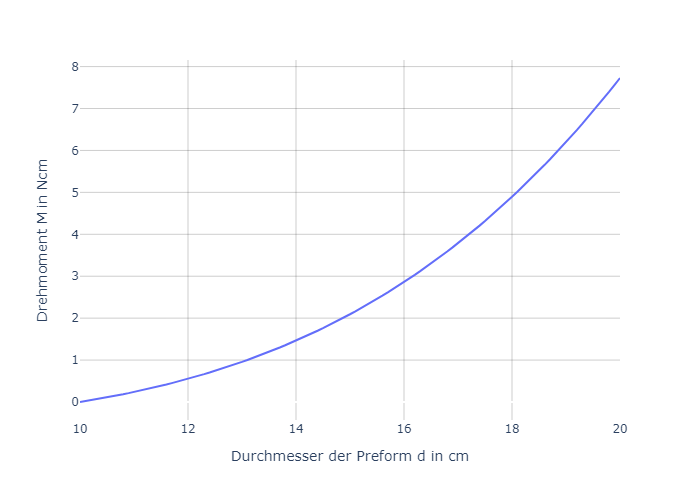
\includegraphics[width = 0.6\textwidth]{Abbildungen/MG_from J.png}
    \caption{Benötigtes Antriebsmoment bei verschieden Füllständen der Spule}
    \label{fig:MG_fromJP}
\end{figure}

Die Abbildung \ref{fig:MG_fromJP} Zeigt den Drehmomentsanstieg für die Beschleunigung bei unterschiedlichen Füllständen der Spule. Das größte Moment was daraus hervorgeht beträgt circa $7,5 Ncm$. Lässt sich für das Drehzahlband kein passender Motor finden ist auch der Einsatz eines Getriebes möglich. Damit der Aufbau möglichst einfach bleibt könnte ein Synchrongetriebe verwendet werde. Diese haben einen hohen Wirkungsgrad und die Übersetzung lässt sich leicht anpassen.
\begin{equation}\label{eq:uebersetzung}
     i=\frac{z_2}{z_1} = \frac{n_1}{n_2} \hspace{10mm} \cite{DIN77212.Juni1989}
\end{equation}

Mit Gleichung \ref{eq:uebersetzung} lässt sich mit der Drehzahl des Motors die Passende Übersetzung berechnen. Synchrongetriebe besitzen einen Wirkungsgrad ($\eta$) der größer als $0,98$ ist \cite{DIN77212.Juni1989}.
\begin{equation}\label{eq:m_synchrongetriebe}
    M_G = M*\frac{z_2}{z_1}\frac{1}{\eta} \hspace{10mm} \cite{DIN77212.Juni1989}
\end{equation}

Das Angepasste Antriebsmoment ($M_G$) ist also von der Zähnezahl der Riemenscheiben abhängig die so berechnet werden müssen das Drehmoment und Drehzahl zu Forderung passen.

%-----vlllt b ab hier ---- auswahl motor%


\subsubsection{Spulenaufnahme}
Die Aufnahme der Spule muss sicherstellen das Sie nicht Durchrutschen kann, da darüber die Kraft auf die Faser wirkt. Da die Spule mit einer Zentralschraube befestigt wird (Abbildung \ref{fig:halbschnitt_Spule}), muss diese das Antriebsmoment aufnehmen können.

\begin{figure}[!h]
    \centering
    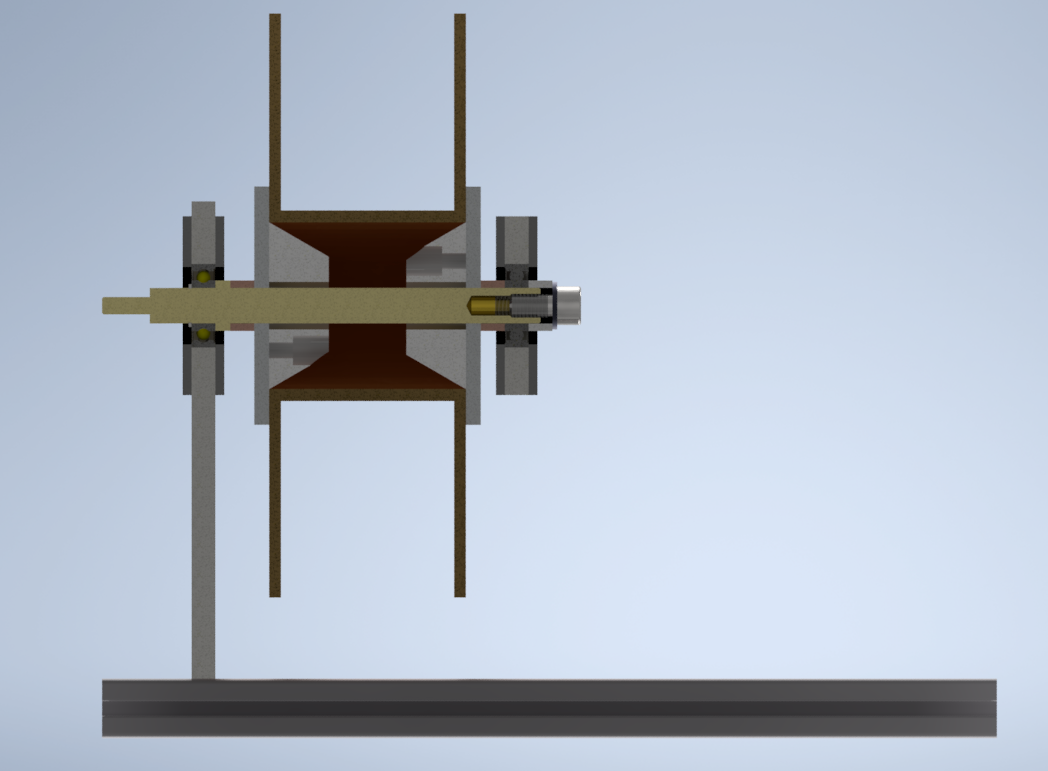
\includegraphics[width = 0.7\textwidth]{Abbildungen/Spulenaufnahme_0.png}
    \caption{Hablschnitt des Abzugs}
    \label{fig:halbschnitt_Spule}
\end{figure}

Um dies Sicherzustellen wird das benötigte Anzugsmoment der Schraube berechnet.
\begin{equation}\label{eq_MA_DIN}
    M_A = F_{Mmax}\cdot(0,16 \cdot P + 0,58\cdot d_2 \cdot \mu_{Gmin} + \frac{D_{KM}}{2}\cdot \mu_{Kmin}) \hspace{10mm} \cite{VDI2230Blatt1.November2015}
\end{equation}

Dabei ist $F_{Mmax}$ die Vorspannkraft der Schraube, welche zum übertragen des Antriebsmomentes benötigt wird. 
\begin{equation}\label{eq_Fmmax}
     F_{Mmax} = \frac{M_{Motor}}{r_a \cdot \mu_{Tmin}} \hspace{10mm} \cite{VDI2230Blatt1.November2015}
\end{equation}
Zur Berechnung wird nun das maximale Drehmoment des Motors ($M_{Motor} = 3Nm$) verwendet, auch wenn dieses viel größer ist als das benötigte Antriebsmoment. Sollte der Motor aus irgendeinem Grund, während des Prozesses, dieses Drehmoment Aufbringen soll sich die Schraubverbindung trotzdem nicht lösen. Unter Verwendung der Haftreibung zwischen Stahl und Stahl ($\mu_{Tmin}$) von circa $0,15$ und dem effektiven Radius ($r_a = 5,25mm$) des Schraubenkopfes der M8 schraube lässt sich die Vorspannkraft und somit auch das Anzugsmoment berechnen. Die Gewindesteigung $P$ beträgt $1,25mm$, der Flankendurchmesser $d_2$ der Schraube beträgt $7,188mm$ und der Wirksame Kopfdurchmesser $D_{KM}$ ist $10,5mm$. Benötigt werden nun nur noch die Haftreibzahl der Kopfauflage ($\mu_{Kmin}$) von $0,15$ und die Haftreibung im Gewinde ($\mu_{Gmin}$) mit einen Wert von $0,12$.
\begin{equation}\label{eq:solve_MA}
        M_A \approx 5,668 Nm
\end{equation}
Da eine M8 8.8 Schraube mit bis zu $24Nm$ belastet werden darf kann die Spule so befestigt werden.


